\documentclass{standalone}
\usepackage[utf8]{inputenc}
\usepackage[english]{babel}
\usepackage{amsmath, amsfonts, amsthm, amssymb, mathtools}
\usepackage[dvipsnames]{xcolor}
\usepackage{graphicx}
\usepackage{anyfontsize}
\usepackage{graphicx, subcaption}
\usepackage{tikz}
\usetikzlibrary{shapes.geometric}
\usepackage{pgfplots}
\pgfplotsset{compat=newest}
\usepgfplotslibrary{statistics}
\usepgfplotslibrary{fillbetween}

\tikzstyle{startstop} = [rectangle, rounded corners, minimum width=3cm, minimum height=1cm, text centered, draw=black, fill=red!30]
\tikzstyle{io} = [trapezium, trapezium left angle=70, trapezium right angle=110, minimum width=3cm, minimum height=1cm, text centered, draw=black, fill=blue!30]
\tikzstyle{process} = [rectangle, minimum width=3cm, minimum height=1cm, text centered, draw=black, fill=orange!30]
\tikzstyle{decision} = [diamond, minimum width=3cm, minimum height=1cm, text centered, draw=black, fill=green!30]
\tikzstyle{arrow} = [thick,->,>=stealth]

\begin{document}
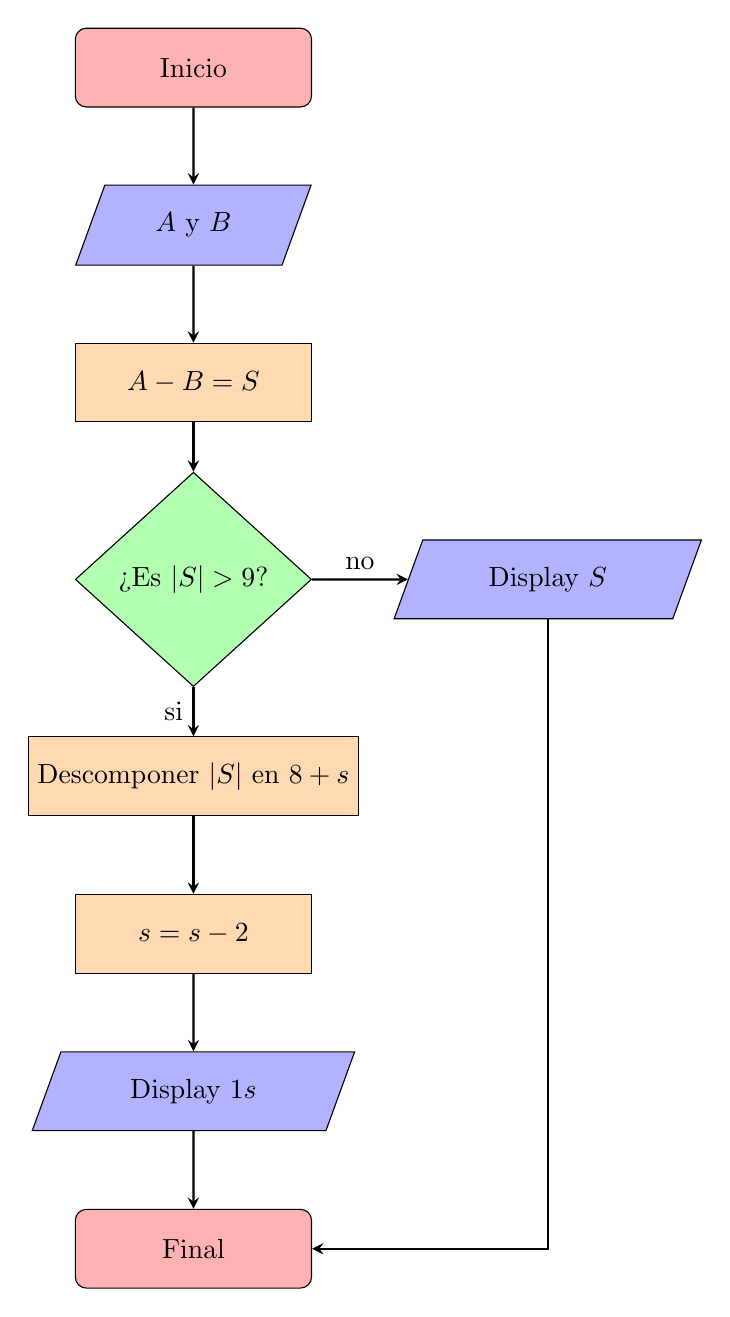
\begin{tikzpicture}[node distance=2cm]
	\node (start) [startstop] {Inicio};
	\node (input) [io, below of=start] {$A$ y $B$};
	\node (A-B) [process, below of=input] {$A - B = S$};
	\node (>9) [decision, below of=A-B, yshift=-0.5cm] {¿Es $|S| > 9$?};
	\node (8+s) [process, below of=>9, yshift=-0.5cm] {Descomponer $|S|$ en $8 + s$};
	\node (outputS) [io, right of=>9, xshift=2.5cm] {Display $S$};
	\node (s-2) [process, below of=8+s] {$s = s - 2$};
	\node (output1s) [io, below of=s-2] {Display $1s$};
	\node (stop) [startstop, below of=output1s] {Final};

	\draw [arrow] (start) -- (input);
	\draw [arrow] (input) -- (A-B);
	\draw [arrow] (A-B) -- (>9);
	\draw [arrow] (>9) -- node[anchor=east] {si} (8+s);
	\draw [arrow] (8+s) -- (s-2);
	\draw [arrow] (s-2) -- (output1s);
	\draw [arrow] (output1s) -- (stop);

	\draw [arrow] (>9) -- node[anchor=south] {no} (outputS);
	\draw [arrow] (outputS) |- (stop);

\end{tikzpicture}

\end{document}
